\documentclass[12pt,a4paper,oneside]{article}
\usepackage{lmodern}
\usepackage[T1]{fontenc}
\usepackage[polish]{babel}
\usepackage{polski}
\usepackage{indentfirst}
\usepackage{enumitem}
\usepackage{fancyhdr}
\usepackage{graphicx}
\usepackage{float}
\setlist{nolistsep}
\pagestyle{fancy}
\selectlanguage{polish}
\setlength{\headheight}{15pt}

% rozszerzenie nieco strony
% \setlength{\topmargin}{-1cm} \setlength{\textheight}{24.5cm}
% \setlength{\textwidth}{17cm} \addtolength{\hoffset}{-1.5cm}
% \setlength{\parindent}{0.5cm} \setlength{\footskip}{2cm}
\linespread{1.2} % odstep pomiedzy wierszami

%%%% ZYWA PAGINA %%%%%%%%%%%
\newcommand{\tl}[1]{\textbf{#1}} 
\pagestyle{fancy}
\renewcommand{\sectionmark}[1]{\markright{\thesection\ #1}}
\fancyhf{} % usuwanie bieżących ustawień
\fancyhead[LE,RO]{\small\bfseries\thepage}
\fancyhead[LO]{\small\bfseries\rightmark}
\fancyhead[RE]{\small\bfseries\leftmark}
\renewcommand{\headrulewidth}{0.5pt}
\renewcommand{\footrulewidth}{0pt}
% \addtolength{\headheight}{0.5pt} % pionowy odstęp na kreskę
\fancypagestyle{plain}{%
\fancyhead{} % usuń p. górne na stronach pozbawionych numeracji
\renewcommand{\headrulewidth}{0pt} % pozioma kreska
}

\begin{document}
{
\begin{titlepage}
    \fancyhf{}
    \headheight=0pt
    \headsep=0pt
    \begin{center}
        \frenchspacing
        \thispagestyle{empty}
        \makeatletter
        \setlength\@fptop{0\p@ \@plus 1fil}
        \begin{figure}
            \centering
            
\includegraphics[width=0.4\textwidth,keepaspectratio]{politechnika_sl_logo_pion_pl_rgb.png}
        \end{figure}
        \makeatother
        {\large
            % Politechnika Śląska\\
            Wydział Informatyki, Elektroniki i Informatyki}

        \vfill
        \textbf{\Huge
            Aplikacja do zarządzania budżetem domowym}
        \vspace*{1\baselineskip}

        {\large \scshape
            Tworzenie Aplikacji Bazodanowych}
        \vfill

        {\small
            \begin{itemize}
                \item[] Mateusz Cudzik\\
                \item[] Jakub Ferens\\
                \item[] Mateusz Górecki\\
                \item[] Szymon Maciąg\\
                \item[] Kajetan Sommer\\
                \item[] Julia Wojciuch
            \end{itemize}
            \vspace*{1\baselineskip}
            % \vspace{0pt plus 0.5fill}

            Gliwice\\
            \today
        }
        \vspace*{0\baselineskip}
    \end{center}
\end{titlepage}
}

\thispagestyle{empty}
\tableofcontents
\newpage

\section{Wstęp}
Celem projektu jest stworzenie aplikacji do zarządzania domowym budżetem i jego
monitorowania. Warunkiem koniecznym jest obsługiwanie logowania, co umożliwi
korzystanie z niej wielu użytkownikom. Aplikacja pozwoli na tworzenie raportów
oraz kategoryzowanie przychodów i wydatków z różnych kont.

\section{Określenie wymagań}
\subsection{Wymagania funkcjonalne}
\begin{itemize}
    % \setlength\itemsep{0.3em}
    \item Obsługa logowania
    \item Kategorie wydatków/przychodów
    \item Kategorie kont
    \item Transakcje między profilami
    \item Generowanie raportów - analiza finansowa
    \item Przechowywanie skanów paragonów/faktur
    \item Przechowywanie dłużników
    \item Informacje przechowywane w bazie danych
    \item Dodawanie profilów członków rodziny do konta (profil dziecka, rodzica
          itd.)
    \item Dodanie konta bankowego i operacji na nim
    \item Obsługa wydatków i przychodów
\end{itemize}

\subsection{Wymagania niefunkcjonalne}
\begin{itemize}
    % \setlength\itemsep{0.3em}
    \item Bezpieczeństwo – okresowe tworzenie kopi zapasowych danych
    \item Zabezpieczenie profili użytkowników hasłem
    \item Hierarchia użytkowników – różne poziomy uprawnień/dostępu,
          ograniczenia dla profilów młodszych użytkowników
    \item Użyteczność – aplikacja z przystępnym i łatwym w obsłudze interfejsem
          zarówno dla starszych jak i młodszych użytkowników
    \item Wieloplatformowość – przypadku aplikacji webowej dostępność z różnych
          urządzeń przy pomocy dowolnego systemu posiadającego przeglądarkę
    \item System/Aplikacja przystosowana do łatwego rozwoju, rozbudowy i
          aktualizacji
    \item Responsywność – odpowiedź aplikacji na działania użytkownika w
          określonym czasie (przykładowo do trzech sekund)
\end{itemize}

\section{Analiza MoSCoW}
\subsection{Must}
\begin{itemize}
    % \setlength\itemsep{0.3em}
    \item Przechowywanie informacji w bazie danych
    \item Dodawanie wydatków i przychodów
    \item Generowanie raportów
    \item Założenie konta i przypisania do niego danych
    \item Informowanie użytkownika o aktualnym stanie konta, który jest
          zmieniany wraz z kolejnymi wpisami o przychodach/wydatkach
\end{itemize}

\subsection{Should}
\begin{itemize}
    % \setlength\itemsep{0.3em}
    \item Przypomnienie hasła
    \item Formularz rejestracji dostępny dla użytkownika
    \item Dzielenie wydatków i przychodów na kategorie
    \item Generowanie raportów z podziałem wydatków/przychodów na kategorie
    \item Operacje zarządzania profilami (dodawanie, usuwanie itd.)
\end{itemize}

\subsection{Could}
\begin{itemize}
    % \setlength\itemsep{0.3em}
    \item Potwierdzenie rejestracji mailem
    \item Edycja informacji o koncie (nazwy użytkownika, hasła, itd.)
    \item Ustawianie cyklicznych/stałych wydatków/przychodów
    \item Transakcje między profilami
    \item Przechowywanie skanów paragonów/faktur
    \item Definiowanie własnych, niestandardowych kategorii
\end{itemize}

\subsection{Won't}
\begin{itemize}
    % \setlength\itemsep{0.3em}
    \item Weryfikacja Captcha
    \item Przechowywanie informacji o dłużnikach
    \item Powiadomienia o przekroczonym budżecie
\end{itemize}

\section{Scenariusze przypadków użycia}
\subsection{Logowanie}
\subsubsection{Scenariusz główny logowania}
\begin{itemize}
    % \setlength\itemsep{0.3em}
    \item Przypadek rozpoczyna się, gdy niezalogowany użytkownik wejdzie
          na stronę
    \item Użytkownik wpisuje swój login oraz hasło
    \item System sprawdza poprawność danych
    \item Użytkownik zostaje przeniesiony do panelu wyboru profilu
    \item Użytkownik wybiera profil.
    \item Wyświetlony zostaje panel sterowania budżetem
    \item Użytkownik zostaje zalogowany
\end{itemize}

\subsubsection{Scenariusze poboczne logowania}
\paragraph{Konto nie istnieje}
\begin{itemize}
    % \setlength\itemsep{0.3em}
    \item Użytkownik zostaje przeniesiony do formularza rejestracji
    \item Użytkownik wprowadza swoje dane
    \item System sprawdza poprawność danych
    \item Konto zostaje utworzone
\end{itemize}

\paragraph{Wybrany profil jest chroniony}
\begin{itemize}
    % \setlength\itemsep{0.3em}
    \item Użytkownik wpisuje PIN
    \item System sprawdza poprawność danych
    \item W przypadku wprowadzenia poprawnego kodu pin scenariusz się kończy,
          w przeciwnym razie użytkownik jest informowany o błędnym kodzie PIN,
          po kilku błędnych próbach nakładana jest czasowa blokada
\end{itemize}

\paragraph{Wybrany profil jest profilem dziecka}
\begin{itemize}
    % \setlength\itemsep{0.3em}
    \item Użytkownikowi wyświetlone zostaje uproszczone GUI
\end{itemize}

\subsection{Dodawanie przychodów/wydatków}
\subsubsection{Scenariusz główny dodawania przychodów/wydatków}
\begin{itemize}
    % \setlength\itemsep{0.3em}
    \item Zalogowany użytkownik decyduje się dodać przychód/wydatek na panelu
          sterowania budżetem
    \item Użytkownik wpisuje kwotę, nazwę własną operacji oraz wybiera jej
          kategorię
    \item Operacja zostaje uwzględniona w budżecie
\end{itemize}

\subsubsection{Scenariusze poboczne dodawania przychodów/wydatków}
\paragraph{Użytkownik dodaje własną kategorię}
\begin{itemize}
    % \setlength\itemsep{0.3em}
    \item Użytkownik podaje nazwę i wybiera kolor
    \item Kategoria zostaje dodana do listy wszystkich kategorii
\end{itemize}

\paragraph{Użytkownik dodaje wydatek przekraczający saldo}
\begin{itemize}
    % \setlength\itemsep{0.3em}
    \item Użytkownik zostaje ostrzeżony za pomocą powiadomienia przed wykonaniem
          operacji
    \item Użytkownik anuluje albo potwierdza wykonanie transakcji
\end{itemize}

\section{Diagram UML}
\begin{figure}[H]
    \rotatebox{90}{
        \begin{minipage}{\textheight}
            \thispagestyle{empty}
            \centering
            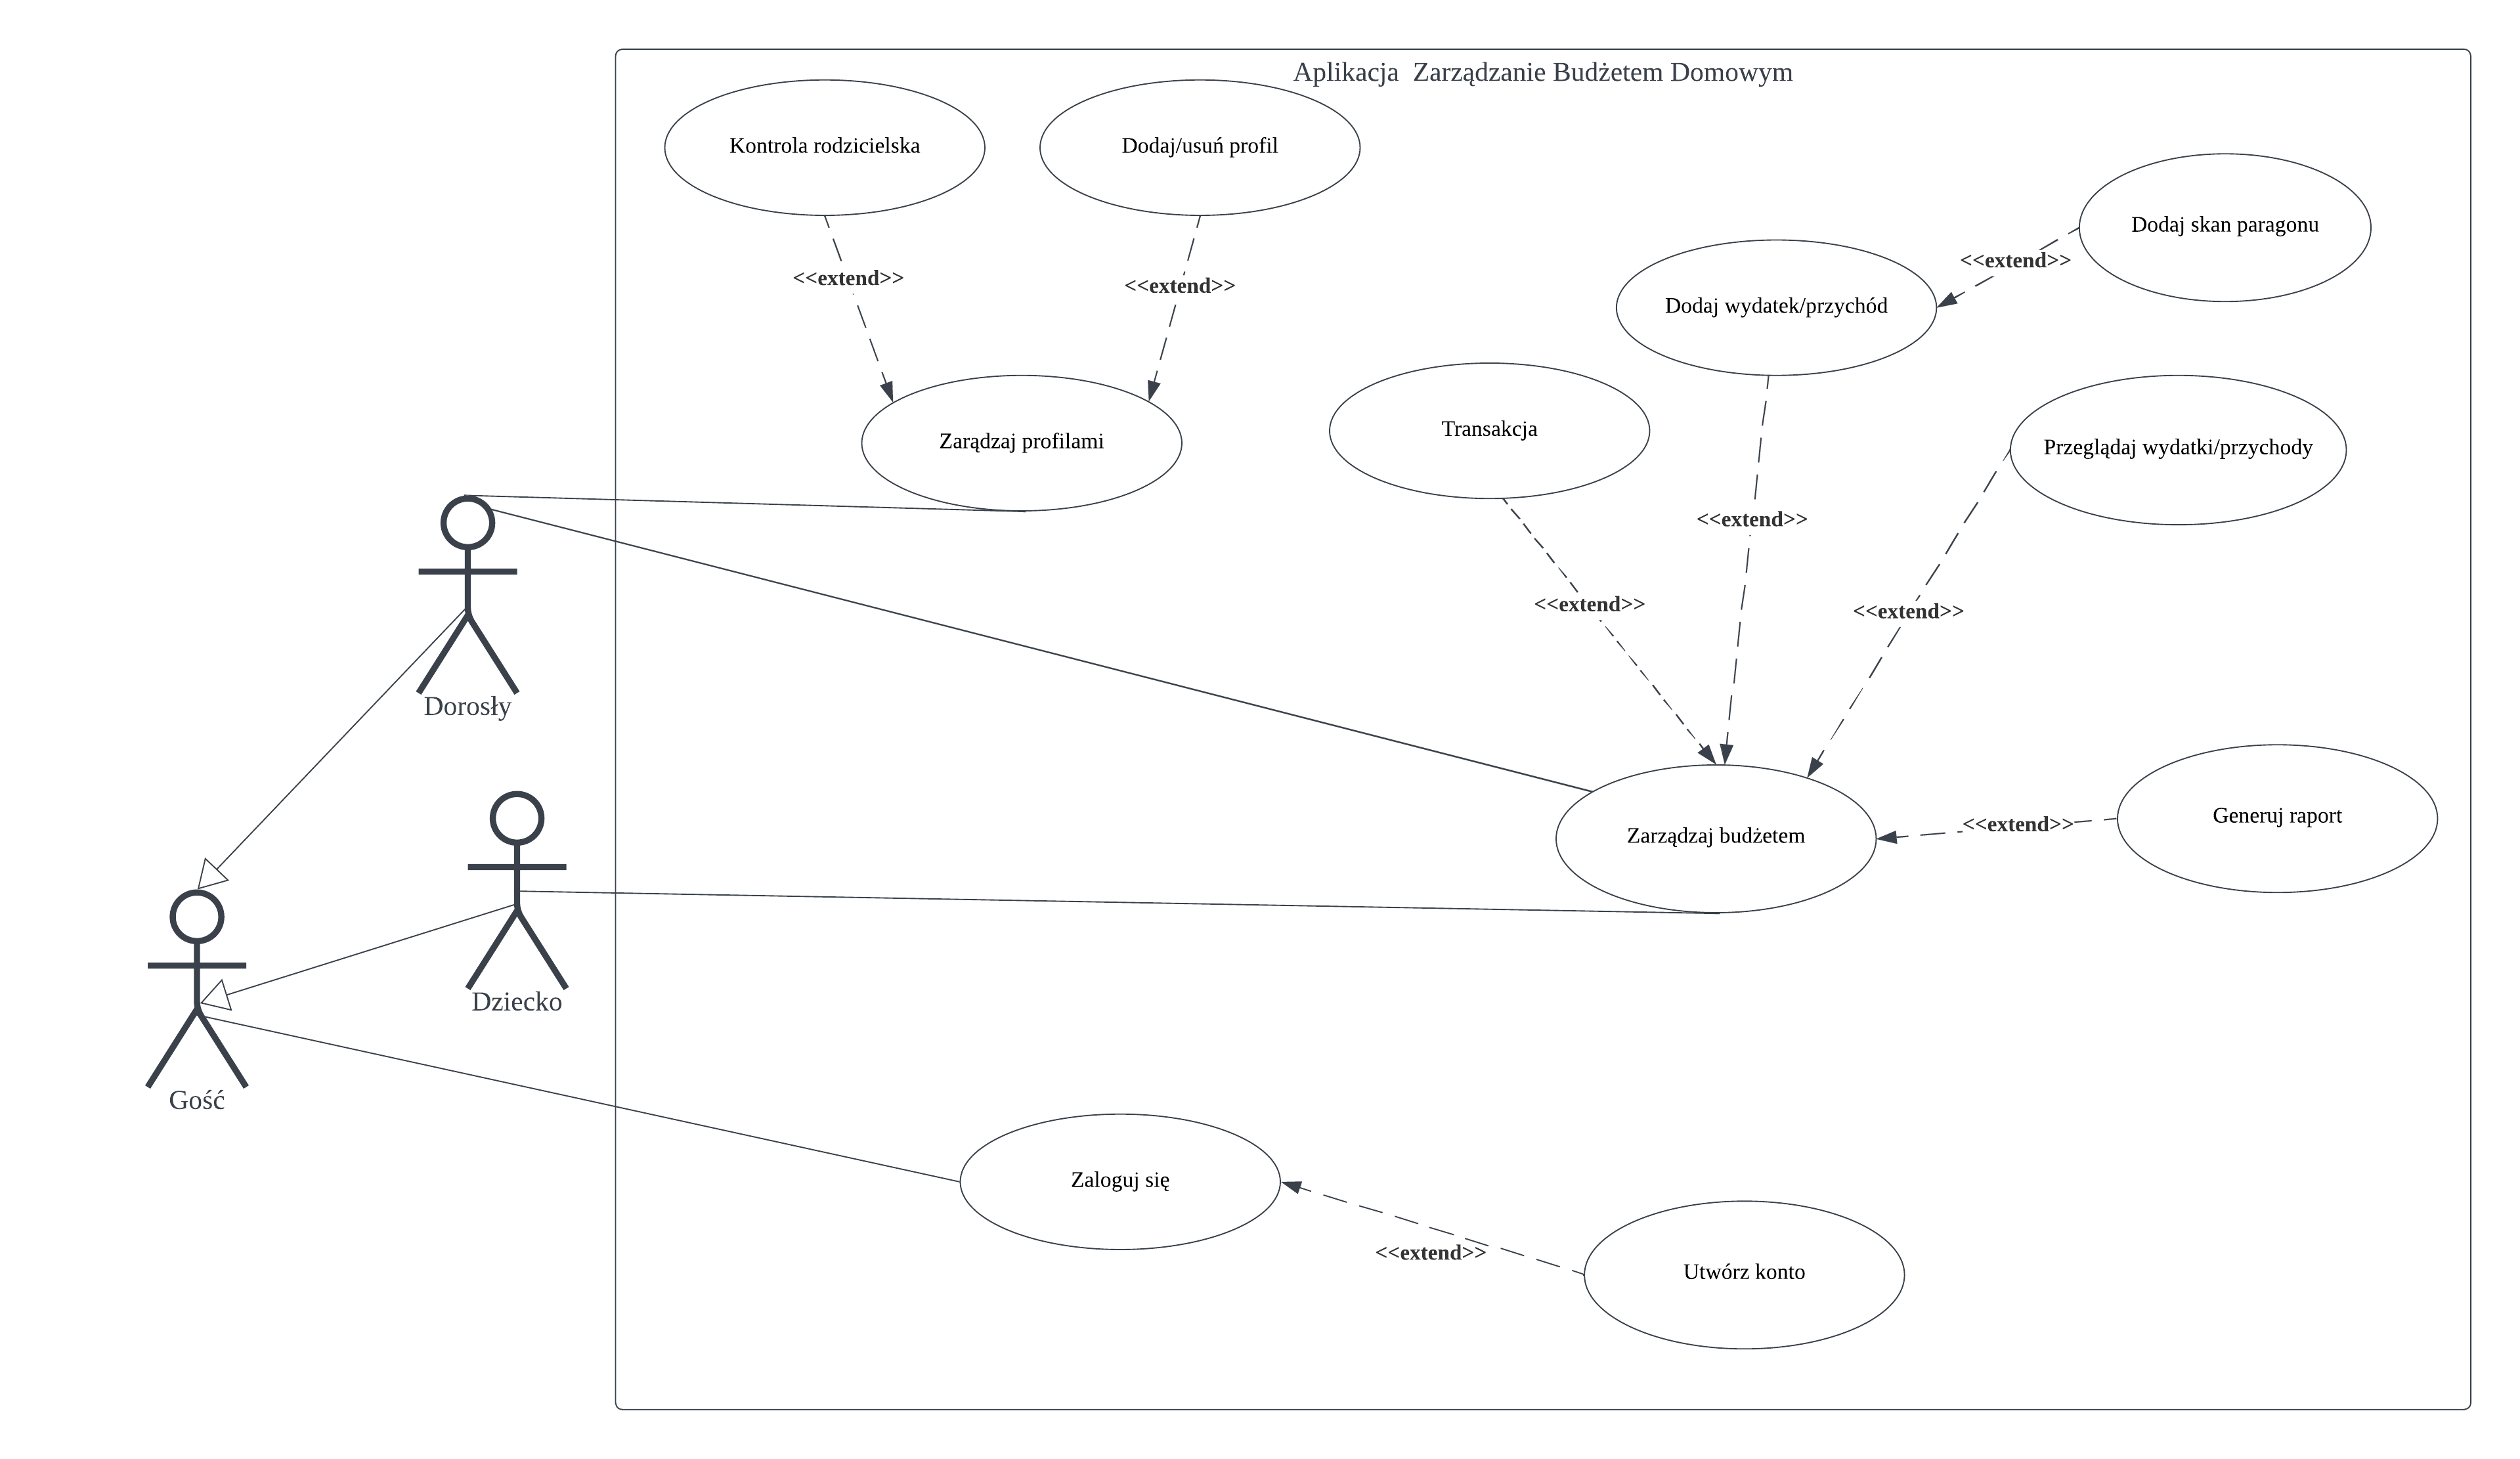
\includegraphics[width=\hsize,keepaspectratio]{UML1.png}
            \caption{Diagram UML}
        \end{minipage}}
\end{figure}

\section{Schemat bazy danych}
\begin{figure}[H]
    \centering
    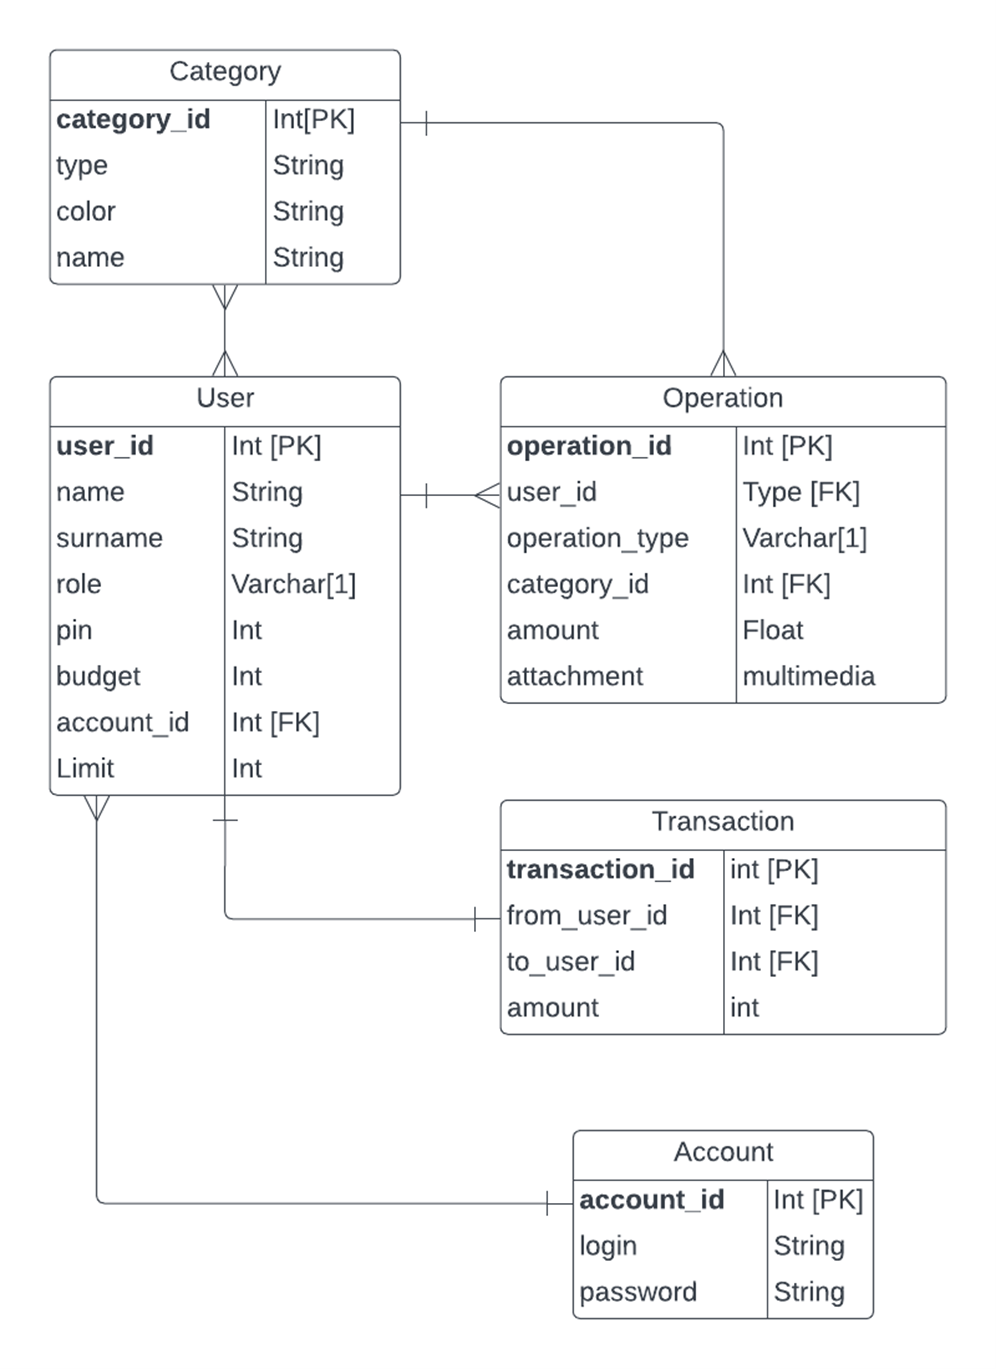
\includegraphics[width=\hsize,keepaspectratio]{DB1.png}
    \caption{Prototypowy schemat bazy danych}
\end{figure}

\section{Specyfikacja zewnętrzna}

\section{Specyfikacja wewnętrzna}

\section{Testowanie i uruchamianie}

\section{Weryfikacja osiągniętych efektów względem założeń}
\subsection{Schemat zaimplementowanej bazy danych}
\begin{figure}[H]
    \centering
    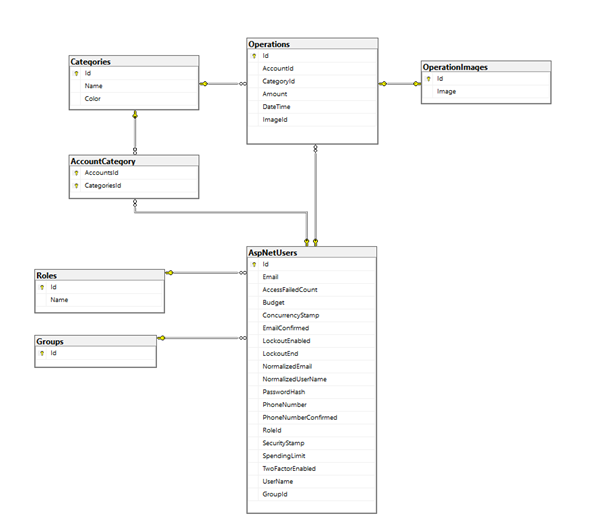
\includegraphics[width=\hsize,keepaspectratio]{DB2.png}
    \caption{Wykorzystany schemat bazy danych}
\end{figure}

\section{Uwagi i wnioski}

\end{document}
